\documentclass[tikz,border=8pt]{standalone}
\usepackage{amsmath}
\usetikzlibrary{arrows.meta,positioning}

\begin{document}
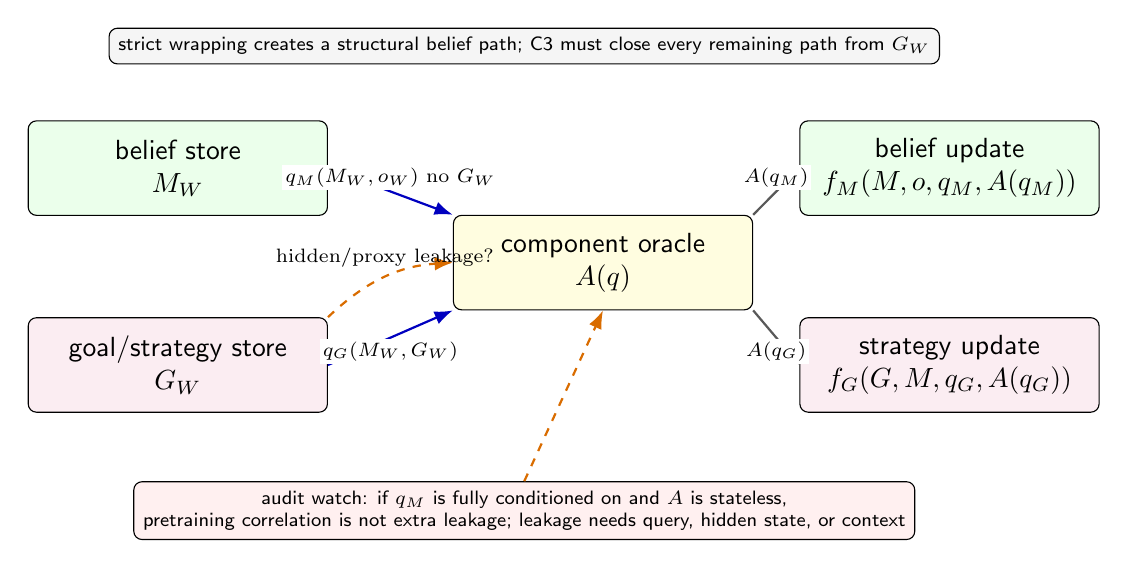
\begin{tikzpicture}[
  font=\sffamily,
  box/.style={draw, rounded corners=3pt, align=center, minimum width=38mm, minimum height=12mm, fill=white},
  note/.style={draw, rounded corners=3pt, align=center, font=\sffamily\scriptsize, fill=white},
  arrow/.style={-Latex, thick, draw=black!65},
  query/.style={-Latex, thick, draw=blue!75!black},
  leak/.style={-Latex, thick, dashed, draw=orange!85!black}
]

\node[box, fill=green!8] (mw) at (-4.4,1.4)
  {belief store\\$M_W$};
\node[box, fill=purple!7] (gw) at (-4.4,-1.1)
  {goal/strategy store\\$G_W$};
\node[box, fill=yellow!12] (comp) at (1.0,0.2)
  {component oracle\\$A(q)$};
\node[box, fill=green!8] (fm) at (5.4,1.4)
  {belief update\\$f_M(M,o,q_M,A(q_M))$};
\node[box, fill=purple!7] (fg) at (5.4,-1.1)
  {strategy update\\$f_G(G,M,q_G,A(q_G))$};

\draw[query] (mw.east) -- node[above, font=\scriptsize, fill=white, inner sep=1pt] {$q_M(M_W,o_W)$ no $G_W$} (comp.north west);
\draw[query] (gw.east) -- node[below, font=\scriptsize, fill=white, inner sep=1pt] {$q_G(M_W,G_W)$} (comp.south west);
\draw[arrow] (comp.north east) -- node[above, font=\scriptsize, fill=white, inner sep=1pt] {$A(q_M)$} (fm.west);
\draw[arrow] (comp.south east) -- node[below, font=\scriptsize, fill=white, inner sep=1pt] {$A(q_G)$} (fg.west);

\draw[leak] (gw.north east) to[bend left=20] node[above, font=\scriptsize] {hidden/proxy leakage?} (comp.west);

\node[note, fill=red!6, minimum width=70mm] (audit) at (0,-2.95)
  {audit watch: if $q_M$ is fully conditioned on and $A$ is stateless,\\pretraining correlation is not extra leakage; leakage needs query, hidden state, or context};
\draw[leak] (audit.north) -- (comp.south);

\node[note, fill=gray!8, minimum width=58mm] at (0,2.95)
  {strict wrapping creates a structural belief path; C3 must close every remaining path from $G_W$};

\end{tikzpicture}
\end{document}
